\documentclass[a4,12pt]{article}

% 畫圖
\usepackage{tikz}
\usetikzlibrary{automata,positioning,arrows}


% 排版
% \usepackage{enumerate}
% \newlist{steps}{enumerate}{1}
% \setlist[steps, 1]{label = Step \arabic*:}

% 中文插件
\usepackage{fontspec}
\usepackage{xeCJK}
\setCJKmainfont{Heiti TC}


% 插入圖片 using \includegraphics[scale = 1]{name.jpg}
\usepackage{graphicx}
\graphicspath{{./picture/}}
\usepackage{float} %设置图片浮动位置的宏包
\usepackage{subfigure}

% \usepackage[]{caption}
% \capto

\usepackage{multicol}

\title{Computer Graphics Hw 3} 
\author{賴柏勛 00957126}

\begin{document}
    \maketitle
    \section{操作方法}

    1、!:up、down

    2、@:left、right

    3、\#:forward、backward

    4、$\$$:pitch

    5、$\%$:yaw

    6、$\^$:roll

    +、-:zoom in、zoom out
   
    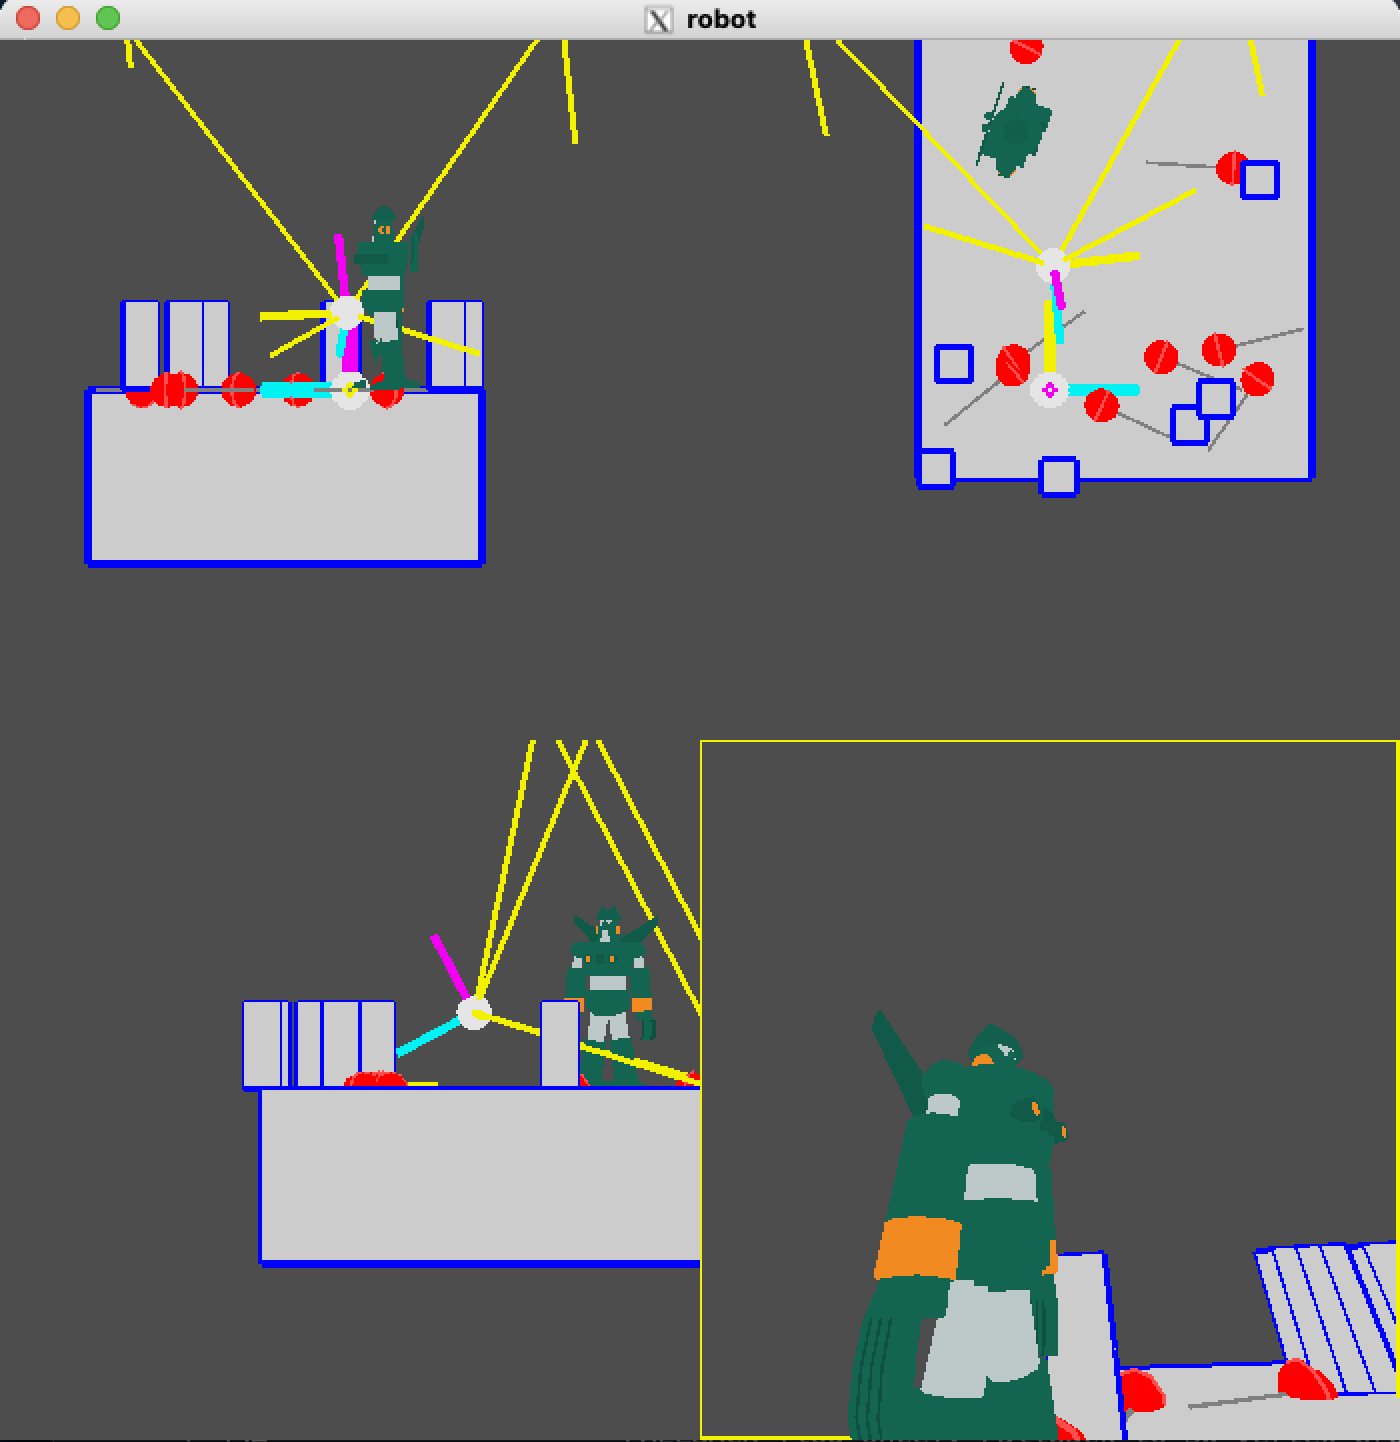
\includegraphics[scale=0.3]{pic.png}
\end{document}